\section{Introduction}
As robots are tasked with challenges of ever-increasing complexity, the need
for a hierarchical system of planning for a goal becomes evident. Such systems
draw clear parallels to the way we plan our own actions: rather than
immediately thinking about the individual muscle motions required to achieve a particular
goal, we apply a top-down approach, first considering at a high level the
steps to be taken, then refining these to lower levels. Recent methods for
hierarchical planning focus on the intersection of high-level task planning
and low-level motion planning. In this framework, the (classical) task planner produces
a symbolic plan containing a sequence of actions to reach a goal
state, and an interface layer refines this plan by sampling concrete values for
the abstract symbols, thus grounding the plan. A central challenge in building such
an interface layer is designing good distributions from which to sample
pose values for the symbolic plan parameters.

\begin{figure}[h]
  \centering
    \noindent
    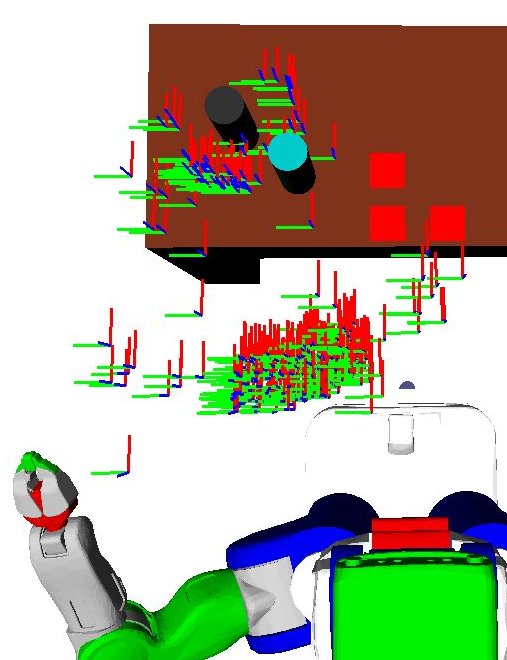
\includegraphics[scale=0.2]{images/move_grasp.png}\hspace{10 mm}
    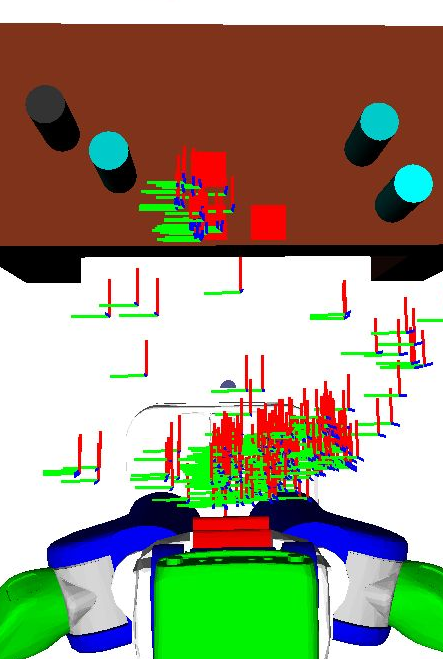
\includegraphics[scale=0.2]{images/move_putdown.png}
  \caption{Screenshots showing some distributions learned by our system in one experimental
    setup. The robot is tasked with grasping the black cylinder and putting it down on the
    central red square. The left image shows learned base motion and grasping distributions,
    and the right shows learned base motion and putdown distributions. The grasp distribution
    properly learned to avoid the region close to the blue obstruction. We sample from these distributions
    to refine the high-level plan, rather than relying on hand-coded generators.}
  \label{fig:cover}
\end{figure}

Our work improves directly upon the interface layer built
by Srivastava et al. They propose a complete backtracking search algorithm for refining
the high-level plan into a set of collision-free trajectories using motion planning, or
propagating symbolic error information back to the task planner if this is not possible.
However, a key limitation of their system is their addressing of the challenge
previously specified; the sampling distributions for
assigning pose values to symbolic parameters are hand-coded, often relying on
geometric information about the object of interest, surrounding objects, and overall
environment. For example, in instantiating an end effector pose for grasping a cylinder off a table,
only the four cardinal directions are attempted, at a fixed height and approach
distance. If all four fail, appropriate error information is returned to the task planner.
This restriction has several negative implications: the parameters of the
hand-coded distributions must be fine-tuned when running the system in a new setting, and the
resulting refinement distributions are discretized, lacking robustness.

Our main contribution is a reinforcement learning approach to find good proposal
distributions for symbolic plan refinement, using rollouts. Our approach allows
the learned distributions to be continuous, robust to changes in the environment, and
trainable for any experimental setting, eliminating the need for distribution parameter tuning. The
introduction of a continuous sampling space for refinement, however, causes the backtracking
search algorithm from Srivastava et al. to lose completeness. Therefore, we also
present a second contribution of our work: randomized refinement, a novel refinement strategy
which maintains at all times a set of instantiations for all plan variables, then randomly
resamples one whose current instantiation is causing a motion planning failure or action precondition
violation. Our randomized refinement strategy allows for a clear formulation of the reinforcement
learning system and naturally guides parameter resampling intelligently, so that better
sampling distributions can be learned more easily for complex environments.

Our algorithm uses an off-the-shelf classical task planner and motion planner, both as black
boxes. An interface layer controls refinement of the classical plan skeleton by assigning continuous pose
values to its symbolic variables and returns failure information to the task planner
when a motion planning feasible refinement is not found within the resource limit. We evaluate
our approach in a variety of test environments involving complicated grasp and putdown
actions with obstructions and base motion. Our experimental results demonstrate noticeable
improvements to both motion planning time and number of calls to the motion planner, as compared
to the hand-coded distributions used in the original system.